\section{Discussion}
\label{sec:discussion}

\subsection{What limits this search}
\label{sec:mmdifferent}

This experiment's most transferable result is not the non-detection but a
measurement of what limits a carrier search at these wavelengths. It is not
depth: the power a transmitter must radiate to cross the threshold here is a
median $\EirpNinetySysMedA$\,W per system, and more power buys nothing at a
frequency the archive never tuned to or never returned to. That inherited
coverage sets the limit.

\emph{Line emission, and not interference, is the astrophysical false positive
here.} Catalogued molecular transitions, almost all of them carbon monoxide,
account for \EvNAttrQp{} of the \EvNCrossQp{} crossings in quality-passing
data, and interference for none (Appendix~\ref{app:rfi}). Of those
attributions \LnAttrSupp{} carry support beyond the frequency match -- a second
transition of the same species, catalogued gas on the sightline, or the
crossing's own recurrence -- while \LnAttrCoincWord{} rest on the coincidence
alone. Lines account for the crossings that stand out and chance for most of
the \EvNUnattrQp{} that remain (\S\ref{sec:trigunif}); the remedy is a
velocity mask in each star's own rest frame (\S\ref{sec:bpicval}). Extended
emission is the second discriminant, with no centimetre analogue: a line
filling the primary beam raises star and control annulus together, and
\DiscFpWin{} of the \DiscFpOfFlags{} windows that reached the spatial stage
are disc or interstellar carbon monoxide (\S\ref{sec:bpicval},
Appendix~\ref{app:falsealarm}).

An illustrative engineering benchmark fixes the scale these limits reach. A
\BenchDiam\,m dish radiating \BenchPowerMW\,MW at \BenchFreqGHz\,GHz with an
aperture efficiency of \BenchEta{} has a directive gain
$G=\eta(\pi D\nu/c)^{2}=\BenchGain$ and so an EIRP of $\BenchEirp$\,W. That is
above the single-epoch crossing limit of \BenchNSysA{} of the \NSysALim{} Class~A
systems that retain unmasked bandwidth. The same gain makes its beam
$\Omega=4\pi/G=\BmOmegaSr$\,sr, illuminating $\BmSkyFrac$ of the sky with a
half-power width of \BmArcsec{} arcsec. These limits therefore apply to beamed
transmitters whose beam contains the Solar System, and EIRP is not transmitter
power.

\emph{The channelisation is inherited.} The carrier search rests on the
\NWinA{} fine-channel windows because almost none of the \NWinB{} coarse ones
can tell a drifting carrier from a stationary one (\S\ref{sec:statistic}). The
widths on offer run from \SzChanFinestKHz\,kHz to \SzChanWidestMHz\,MHz,
\SzChanDexSurvey{} orders of magnitude, or \SzChanDexAll{} beside the
\SzChanLitHz\,Hz channels of centimetre-band carrier searches
(Fig.~\ref{fig:context}(b)), and nothing in the search could choose them.

\emph{Repeat epochs turn a crossing into a testable claim, and an archive
supplies them only incidentally.} Let the \emph{confirmation coverage} $C_{\rm
conf}(\nu)$ be the number of systems toward which two execution blocks of
different observing sessions more than a day apart both cover the sky frequency
$\nu$. A carrier found once there could then have been sought again. It must
be stated against frequency and not as a fraction of the sample, because repeat
visits re-tune and a second epoch is of no use at a frequency it does not
cover. Its support is \CvConfGHzDay\,GHz of union bandwidth, \CvConfPctDay{}
per cent of the \CvUnionA\,GHz searched, falling to \CvConfGHzYr\,GHz beyond a
year. At its best, near \CvConfNuMaxDay\,GHz, it reaches \CvConfNMaxDay{}
systems (Fig.~\ref{fig:waterfall}b). A sensitivity limit and a confirmation limit
are therefore different statements: of the \NSysClassA{} systems,
\ZcConfSysDay{} have a second session covering a frequency of the first more
than a day away and \ZcConfSysYr{} more than a year away, while for the
remaining \ZcNoRepSys{} no transmitted power could have made a confirmation
possible.

%% ★ r27 (R2-D10): the confirmation-coverage figure is row (b) of the merged
%% coverage figure in Sec. 2 (sections/03_sample.tex), which carries the
%% fig:confcov label; make_fig_confcov_v412.py is retired with this float.

\subsection{The search space this archive opens}
\label{sec:newspace}

The one other millimetre search of more than a single line, \citet{Mason2025},
covered \MasonBandMHz\,MHz of Band~3 toward far more distant stars
(\S\ref{sec:intro}). Band~3 is searched here, in \NWinBandThree{} windows down
to \SurvFreqLo\,GHz including $\beta$~Pictoris' CO $J=1\!-\!0$ control.

Union bandwidth overstates what that buys, because different frequencies were
searched toward different numbers of stars and to very different limits.
Figure~\ref{fig:covmap} gives instead the number of independent systems that
would have yielded a recovery at ninety per cent completeness, against sky
frequency and transmitter power. At an EIRP of $\CovEirpRefTex$\,W the covered
frequency falls to \CovUnionAtRef\,GHz, \CovFracAtRef{} per cent of the union.
That coverage reaches \CovNSysAtRef{} systems, and \CovNMaxAtRef{} at the best-covered
frequency near \CovNuMaxAtRef\,GHz. With no limit on power at all, that
frequency reaches \CovNMaxFull{} of the \NSysClassA{} systems, and half the
sample is reached only above $\CovEirpHalf$\,W.

\begin{figure}
\centering
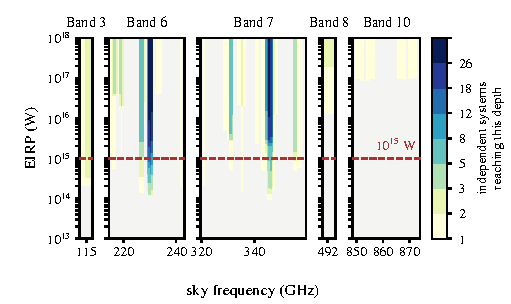
\includegraphics[width=\columnwidth]{figures/completeness_map.pdf}
%% ★ v4.26 (r25-captions): 10 printed lines -> R1 §7's limit of about six.
%% DELETED after checking each: "that is a recovery completeness" restates the
%% clause before it; and "the Class~A union being \CovNIslands{} disjoint
%% islands across \DomAFreqLo--\DomAFreqHi\,GHz" is \S\ref{sec:coverage}'s own
%% sentence, and the abstract's and Conclusion 1's -- all three macros keep
%% two or more citation sites, checked before deleting.
\caption{Where the experiment could have found something. Shading, the
independent systems recovering an unresolved carrier of the plotted EIRP and
sky frequency nine times in ten \emph{in a single epoch}; unshaded, none.
Confirmation needs a second epoch covering the same frequency, which no
power supplies. Panels as in Fig.~\ref{fig:waterfall}b, which gives that coverage.
Dashed, $\CovEirpRefTex$\,W.}
\label{fig:covmap}
\end{figure}

On the continuous-waveform transmitter figure of merit of
\citet{Enriquez2017}, with the single survey-wide fractional bandwidth
replaced by the star-bandwidth product an archive requires, this experiment
is $\CwBareMed$ on the median system and $\CwBareWorst$ on the sample's
largest threshold power.\footnote{The denominator is the star-bandwidth
product $\sum_{i}\Delta\nu_{i}/\nu_{i}$, one term per system, in which
$\Delta\nu_{i}$ is the union of that system's own searched windows and
$\nu_{i}$ the midpoint of the span they cover. It is \CwSigma{} over the
\CwNSys{} systems against \CwUniform{} on a single survey-wide fractional
bandwidth. The two are a factor \CwRatio{} apart because the median system was covered
over only \SysUnionAMed\,GHz of the \CvUnionA\,GHz union. An archive
searches different frequencies toward different stars, which a single
fractional bandwidth credits to every system alike. The published values are
read at the common $\LtCommonSnr\sigma$ threshold of Fig.~\ref{fig:context}, where
\FomLitEnriquez{} becomes \FomLitEnriquezFive{} and \FgLitMargot{} becomes
\FgLitMargotFive. \citet{Margot2023} publish no figure of merit, and the
value quoted here is the same expression on the \FomMargotN{} stars,
\FomMargotLo--\FomMargotHi\,GHz and $\mathrm{EIRP}>\FgMargotEirp$\,W
they do give.} That is a factor $\CwRatioEnriquezFive$ above the
Enriquez value once both are read at the same threshold. It splits into
\CwBandDex{} decades of haystack and \CwEirpDex{} decades of depth: a far
smaller haystack than a wideband centimetre survey of thousands of stars,
and a shallower one.

\subsection{What this experiment excludes, and what it does not}
\label{sec:excludes}

\noindent\emph{What is not constrained.} Every limit here applies to one kind
of signal: an unresolved carrier at the stellar position, confined to a single
\ChanLoA--\ChanHiA\,kHz channel, lying outside the molecular-line mask,
radiating while one of the archival blocks is on sky, and drifting linearly at
no more than its window's ceiling, \DriftCeilLo--\DriftCeilHi\,nHz. The grid
contains every known planet of the sample except \AccelWorstName, whose
windows carry a widened grid reaching it only to the precision its host's mass
and orbit are known (\S\ref{sec:statistic}), but a transmitter on a
rapidly rotating planet spends most of its reach on spin alone
(Fig.~\ref{fig:accel}). Emission broader than a channel needs close to
\ScNBroadRatio$\times$ the power for a feature as wide as the widest line in
these fields, and a carrier on for part of a block comes back at that fraction
of its amplitude. The result is a non-detection and not an exclusion of
persistent transmitters: where the archive observed a frequency once no power
makes a confirmation possible; a shallow repeat tests nothing, as for
\HjNPowerLo{} of the \RcNExcl{} crossings read at a predicted cell; and the
single-cell reading tests only a carrier returning to the same stellar-frame
frequency, which an intermittent, accelerating or deliberately re-tuned
transmitter need not do (\S\ref{sec:etacrv}). Nothing is constrained inside
the $\pm\MaskHalfKms$\,km\,s$^{-1}$ mask, or toward the stars within 40\,pc
that ALMA has not observed, almost all of the \NGaiaCensus{} this volume holds.

\noindent\emph{Two blind spots.} The analysis forms
$(\mathrm{XX}+\mathrm{YY})/2$, which retains the full intensity of a circularly
polarised carrier. The loss is not sensitivity but the discrimination
polarisation would offer against unpolarised astrophysical emission.
ALMA's feeds are linear, and the circularity lies in the cross-hands, which this
analysis does not extract. The frequency coverage, too, is the archive's and not a
choice. The \SbPriorFreqGHz\,GHz positronium hyperfine line that
\citet{Steffes1994} and \citet{Mauersberger1996} observed lies in ALMA Band~5.
This survey holds \LnBFiveWin{} coarse-channel windows there, all toward
\LnBFiveStars, and none of them covers it.

\subsection{What a dedicated ALMA technosignature experiment should do
differently}
\label{sec:future}

The changes a purpose-built experiment on the same telescope needs follow from
the limitations above.

\begin{itemize}[leftmargin=1.2em,itemsep=2pt,topsep=3pt,parsep=0pt]
\item \emph{Channelise finely everywhere.} The \NCoarse{} coarse-channel
windows cannot carry a carrier search at all.
\item \emph{Choose the targets and the frequencies.} An archive weighted
toward dusty discs is the worst case for molecular-line confusion. The
M~dwarfs that dominate the nearby habitable-zone planet census are the least
covered. Windows placed deliberately away from the bright transitions
would recover most of the \MkMaskAGHz\,GHz of the \CvUnionA\,GHz Class~A
union that the mask costs.
\item \emph{Repeat the epochs on purpose, at the same tuning.} Two or three
visits separated by days and by years turn a crossing into a testable claim,
and the separation is a scheduling constraint rather than extra sensitivity
(Fig.~\ref{fig:waterfall}b). Two epochs cannot test an orbit, only fit one.
Three separated epochs over-determine it, and \PaNSysThree{} of the
\NSysClassA{} systems here already carry three at a common frequency. The
shortfall is therefore not coverage but a candidate seen at more than one of them.
\item \emph{Retain the visibilities.} Rotating the phase centre to the star
leaves a genuine point source entirely in the real part of the visibility.
A test on that part asks whether the data contain a source where the star is, a stronger
question than any rank against neighbouring positions in an image.
\end{itemize}
